% \documentclass[xcolor=dvipsnames,10pt]{beamer}
% \documentclass[10pt,xcolor=dvipsnames]{beamer}
\documentclass[hyperref={pdfpagelayout=SinglePage}]{beamer}
\usepackage[usestackEOL]{stackengine}
% \documentclass{beamer}
% \usepackage{fontspec}
\usepackage[utf8]{inputenc} 
\usepackage{pbsi}
\usepackage[T1]{fontenc}
% \usepackage[frenchb]{babel}
\usepackage{setspace}
\usepackage{xcolor}
\usepackage{listings}
\lstset
{
    language=[LaTeX]TeX,
    breaklines=true,
    basicstyle=\tt\scriptsize,
    keywordstyle=\color{black},
    identifierstyle=\color{black},
}

\def\tcb{\color{blue}}

% \AtBeginSection[]{
%   % \begin{frame}
%   % \vfill
%   % \centering
%   % \begin{beamercolorbox}[sep=8pt,center,shadow=true,rounded=true]{title}
%   %   \usebeamerfont{title}\insertsectionhead\par%
%   % \end{beamercolorbox}
%   % \vfill
%   % \end{frame}
% }
\graphicspath{ {tikz/} }


% \usepackage{beamerthemebars}
% \usepackage[bars]{beamerthemetree}
\usepackage{tkz-euclide}
\usetkzobj{all} 

\usepackage{multicol}

\usepackage{appendixnumberbeamer}
\usepackage[framed,autolinebreaks,useliterate]{mcode}%
\usepackage{listings}
% \setbeamercovered{highly dynamic}
% \input{mypackagebeamer}
% \input{definitions}

\usepackage{tikz}
\usetheme{Dresden}
% \usetheme{default}
%\usecolortheme{lily}
\useoutertheme[subsection=false]{smoothbars}
%\useoutertheme[subsection=false]{miniframes}
\useinnertheme{circles}
\usefonttheme[onlymath]{serif}
\setbeamertemplate{navigation symbols}
%\setRL
%\insertslidenavigationsymbol

\setbeamertemplate{footline}[frame number]


\setbeamersize{text margin left=0.5cm,text margin right=0.5cm}
\setbeamersize{text margin left=0.5cm}
% \usepackage{beamerthemebars}
% \usepackage[bars]{beamerthemetree}
% \setbeamercovered{higly dynamic}
%% ================== block: Information ==========================
% \setbeamertemplate{footline}[body]
% \title[]{DFDL: \\Discriminative Feature-oriented \\Dictionary Learning \\for Histopathological Image Classification}
% \subtitle{}
% \author[]{\small Tiep Huu Vu\\ \tcb{Master Paper Presentation}\\
% \vspace{3mm} \includegraphics[scale=0.3]{figs/ipal.png}  }

% \date[]{
% \vspace{3mm} April 9, 2015}
% \institute[]{Department of Electrical Engineering \\  \vspace{2mm}Pennsylvania State University }
%% ------------------end of block: Information ----------------------------

\def\changemargin#1#2{\list{}{\rightmargin#2\leftmargin#1}\item[]}
\let\endchangemargin=\endlist 

\def\mylatex{\textrm{\LaTeX~}}

\setbeamertemplate{navigation symbols}{}

%% ================== commands ==========================
\newcommand{\myShowPoints}[2]{
\tkzDrawPoints(#1) \tkzLabelPoints[#2](#1)
}   

\newcommand{\myGetMidPoint}[3]{
\tkzDefMidPoint(#1,#2)\tkzGetPoint{#3}
}   
%% ------------------ end of commands -------------------
  %%%%Title Slide{
\title[Discriminative Dictionary Learning]{\LaTeX ~basics}
\subtitle{}
\author[Tiep Huu Vu]{Drawing geometric objects with \href{http://www.altermundus.fr/downloads/documents/Sangaku.pdf}{tkz-euclide} package}
\titlegraphic{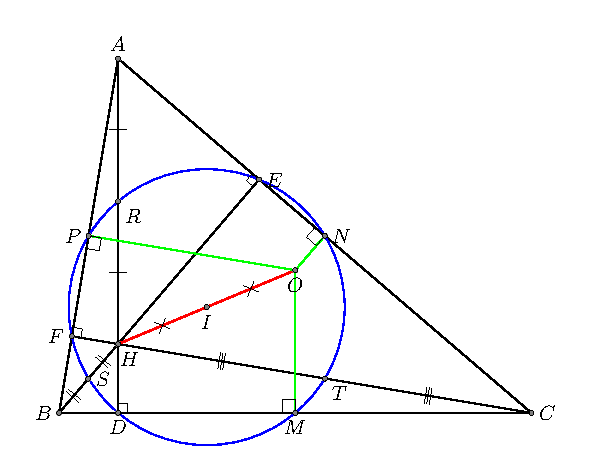
\includegraphics[height=4.5cm]{triangle_euler.pdf}} % instead of \logo 
\institute {\\
\par Tiep Vu Huu\\ \vspace{4mm}}

\begin{document}
%----------- titlepage ----------------------------------------------%
% \begin{frame}[plain]
%   \titlepage 
% \end{frame}

{
\usebackgroundtemplate{\includegraphics[width=\paperwidth]{tikz/background_figures.pdf}}%
\begin{frame}[plain]
\end{frame}
}
% section online_editors (end)
% \def\bfblue{\textbf{\t}}
% =========================== New Slide =================================
\begin{frame}[fragile]
\frametitle{Why are figures important?}
\begin{center}
    {\textbf{\tcb``A picture is worth a thousand words''}}
\end{center}

\begin{columns}
    \begin{column}{0.6\textwidth}

        Why are figures important?
        \begin{itemize}
            \item Explain difficult models.
            \item Visualize your idea.
            \item Show the results.
            \item Can be reused in slides and posters
            \item Readers look at figures first. 
            \item Reflect your respect to your own works.
            \item ...
        \end{itemize}

    \end{column}

    \begin{column}{0.4\textwidth}
    \begin{figure}
        \includegraphics[scale = .35]{figs/pythagoreantheorem.png}
    \end{figure}
    \end{column}
\end{columns}

% $\Rightarrow$ \tcb{\bf Treat graphics as first-class citizens of your papers\footnote{\footnotesize \href{https://www.bu.edu/math/files/2013/08/tikzpgfmanual.pdf}{TikZ pgf manual}}}
$\Rightarrow$ \tcb{\bf Treat graphics as first-class citizens of your papers} 
\\
Source: \href{https://www.bu.edu/math/files/2013/08/tikzpgfmanual.pdf}{\tcb TikZ pgf manual}

\end{frame}



% =========================== New Slide =================================
\begin{frame}[fragile]
\frametitle{Important factors on good figures/charts/diagrams}

What factors affect figure's quality? (Including but not limited to):
\begin{columns}
    \begin{column}{0.6\textwidth}
    \begin{enumerate}
        \item Resolution (I prefer {\tcb vector graphics}).
        \item Display well on several platforms (phones, computers, projectors, printers).
        \item {\tiny Font size}, \textrm{font family}.
        \item Consistent with your main texts. \tikz \node [draw] at (0,0) {y = Dx}; ,$y = Dx, \mathbf{y} = \mathbf{Dx}$. 
        \item {\color{yellow} Colors}, markers: $\bullet, \blacksquare, \triangle$.
        \item Line thickness: \tikz \draw [ultra thick, blue] (0,0) -- (1, 0); \tikz [red]\draw (0,0) -- (.5, 0);.
        \item Labels, legends, captions.
        \item File size (not too big).
        \item No distracted information.
    \end{enumerate}

    \end{column}

    \begin{column}{0.4\textwidth}
    \begin{figure}
        \includegraphics[scale = .15]{figs/chart-type-front.png}
    \end{figure}
    \end{column}
\end{columns}
\end{frame}
% =========================== New Slide =================================
\begin{frame}[fragile]
\frametitle{Font family}
\begin{columns}
    
    \begin{column}{0.5\textwidth}
    \begin{center}
        \textrm{Serif font (e.g. Time Roman)}  
    \framebox{\Longstack[l]{\textrm{\centering The quick brown fox jumps} \\ \textrm{\centering over the lazy dog.}}}
    \end{center}
    \begin{itemize}
        \item Good for: 
            \begin{itemize}
                \item Paragraphs,
                \item Prints.
            \end{itemize}
        \item Bad for:
            \begin{itemize}
                \item Labeling,
                \item Short strings of text,
                \item Slides or posters.
            \end{itemize}
    \end{itemize}
    \end{column}

    \begin{column}{0.5\textwidth}
    \begin{center}
        Sans-serif (e.g. Arial)\\
    \framebox{\Longstack[l]{\textsf{\centering The quick brown fox jumps} \\ \textsf{\centering over the lazy dog.}}}
    \end{center}
    \begin{itemize}
        \item Good for:
            \begin{itemize}
                \item Labeling,
                \item Short string of text,
                \item Projector.
            \end{itemize}
            {\tcb$\Rightarrow$ good for figures.}
        \item Bad for: 
            \begin{itemize}
                \item Paragraphs.
            \end{itemize}
    \end{itemize}
    \end{column}
\end{columns}
\begin{center}
{\large\bsifamily{Don't use rare f$\blacksquare$nts.}}
    
\end{center}
\end{frame}


% =========================== New Slide =================================
\begin{frame}[fragile]
\frametitle{Font size}

% \begin{columns}
% 
    % \begin{column}{0.5\textwidth}
    \begin{figure}
    \centering
        \includegraphics[scale = .35]{figs/bad_fontsize2.png}
    \end{figure}
    Text in figure is too small compared to the caption and main text. 
%     \end{column}
%     \begin{column}{0.5\textwidth}
%     \begin{itemize}
%         \item aa
%     \end{itemize}

%     \end{column}
% \end{columns}
\end{frame}

% =========================== New Slide =================================
\begin{frame}[fragile]
\frametitle{Colors, markers}

\begin{columns}

    \begin{column}{0.5\textwidth}
    \begin{figure}
        \includegraphics[scale = .3]{figs/bad_color.png}
    \end{figure}
    \end{column}
    \begin{column}{0.4\textwidth}
    \begin{itemize}
        \item Colors look similar (not good for black-white print, colorblind people)
        \item Should choose different markers ($\bullet, \square,\blacksquare, \triangle$) for each line. 
    \end{itemize}

    \end{column}
\end{columns}
\end{frame}

% =========================== New Slide =================================
\begin{frame}[fragile]
\frametitle{A good plot}

\begin{columns}

    \begin{column}{0.5\textwidth}
    \begin{figure}
        \includegraphics[scale = .3]{figs/good_plot.png}
    \end{figure}
    \end{column}
    \begin{column}{0.4\textwidth}
    \begin{itemize}
        \item Good ratio of font size (in ticks, labels, legends).
        \item Good choice of color.
        \item Good choice of line type (dashed, solid).
    \end{itemize}

    \end{column}
\end{columns}
Source: \href{http://www.mrl.ucsb.edu/~seshadri/PreparingFigures.pdf}{\tcb Preparing figures for publication and presentations.}
\end{frame}

% =========================== New Slide =================================
\begin{frame}[fragile]
\frametitle{A bad plot}

\begin{columns}

    \begin{column}{0.5\textwidth}
    \begin{figure}
        \includegraphics[scale = .3]{figs/bad_tick.png}
    \end{figure}
    \end{column}
    \begin{column}{0.4\textwidth}
    \begin{itemize}
        \item Bad ratio of font size (in ticks, labels, legends).
        \item Bad choice of color.
        \item Bad choice of line type.
        \itme Font types are different.
    \end{itemize}

    \end{column}
\end{columns}
Source: \href{http://www.mrl.ucsb.edu/~seshadri/PreparingFigures.pdf}{\tcb Preparing figures for publication and presentations.}
\end{frame}

% =========================== New Slide =================================
\begin{frame}[fragile]
\frametitle{Color selection}

\begin{columns}

    \begin{column}{0.4\textwidth}
    \begin{figure}
        \includegraphics[scale = .3]{figs/bad_tick.png}
    \end{figure}
    \end{column}
    \begin{column}{0.6\textwidth}
    \begin{itemize}
        \item Different font size/family in labels, legends and ticks.
        \item Redundant ticks.
        \item Bad choice of colors and line type.
    \end{itemize}

    \end{column}
\end{columns}
\end{frame}

% =========================== New Slide =================================
\begin{frame}[fragile]
\frametitle{Another good plot}

\begin{columns}

    \begin{column}{0.6\textwidth}
    \begin{figure}
        \includegraphics[scale = .3]{figs/good_plot1.png}
    \end{figure}
    \end{column}
    \begin{column}{0.4\textwidth}
    \begin{itemize}
        \item Font size/family
        \item Markers, line thickness, Colors
        \item Focus on main methods.
    \end{itemize}

    \end{column}
\end{columns}
\end{frame}

% =========================== New Slide =================================
\begin{frame}
\frametitle{Don't abuse 3D figures}
\begin{center}
\includegraphics[width = .9\textwidth]{figs/bad1.png}
\end{center}
\begin{itemize}
    \item Smaller parts look bigger and vice verse (3D-distorted proportions). 
    \item Color choice (do not apply color randomly).
    \item The shadings add nothing ``information-wise''
\end{itemize}
Source: \href{https://www.bu.edu/math/files/2013/08/tikzpgfmanual.pdf}{\tcb TikZ and pgf Manual}
\end{frame}



% =========================== New Slide =================================
\begin{frame}
\frametitle{Softwares for generating good figures}
\begin{itemize}
    \item MS Office Excel, Visio. 
    \item MATLAB.
    \item \href{https://www.r-project.org/}{\tcb R} (a programming language).
    \item \href{http://matplotlib.org/}{\tcb matplotlib} (a Python package for plotting).
    \item \href{https://imagej.nih.gov/ij/}{\tcb ImageJ}
    \item \href{https://www.geogebra.org/}{\tcb GeoGebra}
    \item \href{https://inkscape.org/en/}{\tcb Inkscape}
    \item \href{http://pgfplots.sourceforge.net/gallery.html}{\tcb TikZ and pgfplot} (a package in \mylatex).
    \begin{itemize}
        \item Free, lightweight, no need more installation if you have \mylatex
        \item Highly Customizable.
        \item Takes time to generate figures, but figures are easily edited later (in any text editor). 
        \item Generate vector-graphic, small-file-size figures.
    \end{itemize}
\end{itemize}
\end{frame}
% =========================== New Slide =================================
\begin{frame}
\frametitle{Some TikZ examples}
\begin{center}
\includegraphics[width = .9\textwidth]{tikz/ibladlprocedure_step1.pdf}
\end{center}
\end{frame}

% =========================== New Slide =================================
\begin{frame}
\frametitle{Some TikZ examples}
\begin{center}
\includegraphics[width = .7\textwidth]{tikz/compare_shared.pdf}
\end{center}
\end{frame}
% =========================== New Slide =================================
\begin{frame}
\frametitle{References}
\begin{itemize}
    \item \href{https://www.bu.edu/math/files/2013/08/tikzpgfmanual.pdf}{\tcb TikZ and pgf Manual}
    \item \href{http://www.mrl.ucsb.edu/~seshadri/PreparingFigures.pdf}{\tcb Preparing figures for publication and presentations.} (Ram Seshadri, UCSB).
    \item \href{http://journals.plos.org/ploscompbiol/article?id=10.1371/journal.pcbi.1003833}{\tcb 10 simple rules for better figures}
\end{itemize}

\end{frame}















% =========================== New Slide =================================

  \begin{frame}
  \vfill
  \centering
  \begin{beamercolorbox}[sep=8pt,center,shadow=true,rounded=true]{title}
    \usebeamerfont{title} Thanks for watching%
  \end{beamercolorbox}
  \vfill
  \end{frame}
\end{document}
